\documentclass[11pt]{article}
\usepackage{amsmath}
\usepackage{amssymb}
\usepackage{amscd}
\usepackage{biblatex}
\addbibresource{bibliography.bib}
\usepackage{graphicx}
\usepackage{euler}

\graphicspath{ {./images/} }
\title{Neural network knowledge distillation in tensor networks}
\author{Dereck Piché}
\date{\today}

\begin{document}
\maketitle
\begin{abstract}
\end{abstract}

\section{Introduction}
TODO


\section{Knowledge Distillation}
Knowledge Distillation is a machine learning practice which involves
taking a trained model and using it's parameters to train another one.
The already trained model is referred to as the "teacher", and 
the model in which his "knowledge" is to be distilled is referred to as
the "student".

\subsection{Response-Based Knowledge Distillation}
While this is a relatively novel technique, there are 
already several distinct approaches introduced by researchers.
We used two of these approaches. Our inspiration for the distillation 
methodology was found in a a 2021 survey which resumed the emerging practice \textcite{Gou_2021}


The first approach we used to look exclusively at the outputs
of the student and teacher. Now, we apply the logits
of our functions element-wise to the outputs and the softmax.
\begin{equation}
    softmax(v_i) = \frac{e^{v_i}}{\sum_{j}{e^{v_i}}}
\end{equation}
The softmax function's objective is to transform the logits
into probability distributions for the different classes.
We will now apply a loss function $L$ to these two functions.
Since we are trying to reduce the divergence between 
two distributions, we will use the Kullback-Leibler divergence loss
\begin{equation}
    KL(P, Q) = \frac{1}{n} \sum_i^n Q \frac{log_e(Q)}{log_e(P)}
\end{equation}
Here, $Q$ is the distribution we are aiming for and $P$ is the one we have.



\section{Tensor Networks}
Tensor Networks come from the study of quantum phenomena. They 
started being used recently as machine learning models. Tensor Networks
can be thought out as two things: a visual notation system and a 
set of methods for tensor manipulation. 

\paragraph{Tensors}
Before explaining these two, we shall 
disambiguate the meaning of "tensor". In this report (and very often in the context
of machine learning), we use the word "tensor" to refer to the mathematical arrays
of arbitrary indices. Here, the number of indices is called the "order" of the 
tensor, meaning that vectors are simply tensors of order $1$ and matrices tensors 
of order $2$. 

\paragraph{Contraction}
At the heart of tensor networks is the {\it contraction} operation.
Tensor Networks are used to compute a larger network by "contracting" several
smaller tensors over chosen indices. A "contraction" is simply an operation 
where we sum over indices. For example, the contraction of $A_{ijk}$ and 
$B_{ijk}$ on index $j$ will produce the tensor $C_{ik} = \sum_{j} A_{ijk} B_{ijk}$.
Evidently, the two indices present in a contraction must be of the same size.

\paragraph{Notational system}
The principal motivation behind the creation of Tensor Networks 
to compute or approximate large tensors {\it contracting} several
smaller tensors over chosen indices. This is all well and good until 
our conventional summation notation begins overclocking our primal brains.
So, in order to make the manipulation of these network of tensors, mathematicians
created a notational system. Tensors are represented as nodes where each 
vertex connected to the node represents one of the tensor's indices. 
If a vertex connects two nodes, it means that the indices shall be contracted 
in order to produce the post-contraction tensor. It should be evident that
by the definitions above, no node (tensor) is completely isolated in a tensor network,
as it would be completely purposeless. The shape of the post-contraction tensor 
can be easily visually identified, since it is found in the unconnected vertices.
A simple tensor network can be found in figure \ref{fig:tensor_net}.

\paragraph{Tensor Network Methods}
The term {\it Tensor Network Methods} is used to refer to, you guessed it, the methods.
There are several architectures of Tensor Networks that are frequently used, such 
as the {\it Matrix Product State (MPS)}, the {\it Tenso}

\begin{figure}[h]
\centering
\caption{Simple tensor network illustrating the notation.}
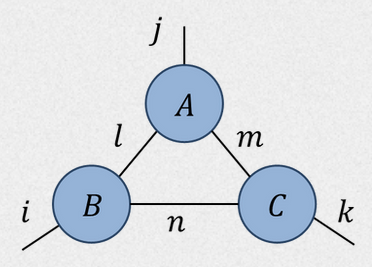
\includegraphics[width=0.5\textwidth]{images/2023-03-21-10-22-39.png}
\label{fig:tensor_net}
\end{figure}

\subsection{Tensor Products and Transformations}

Consider an input vector $x \in R^d$. Let $\phi(x) : R \mapsto R^{d_{\phi}}$.  
Then, let us take the tensor product of apply $\phi(x)$ applied 
to every element of the vector $x$.
\begin{equation}
    \Phi(x) = \phi(x_1) \otimes  \phi(x_2) 
                \otimes (\dots) \phi(x_d)
\end{equation}
We obtain a tensor $\Phi(x)$, of which the sum of it's element 
contain the basis of a space of products of the elements of the transformed
elements of $\phi(x)$.

In order to reduce the abstractness of this statement, we can take say
that $\otimes$ refers to the Kronecker Product.

A particular dimension is of interest here, the transformation

\begin{equation}
    \phi(x) = 
    \begin{bmatrix}
        1 \\
        x
    \end{bmatrix}
\end{equation}
With, this particular transformation, the Kronecker Product gives us a 
$\Phi(x)$ which is a matrix where each element is a basis of the 
space of multilinear functions on the elements of the vector $x$.

\subsection{Linear Combinations}
How do we use $\Phi(x)$, how does it become useful? Well, it becomes useful 
when we take a linear map of it's elements. Let our $\Phi(x)$ be an 
arbitrarily shaped tensor of $d_{\Phi}$ dimensions. The final form of our 
function $f(x)$ will be
\begin{equation}
    f(x) = \sum_{i}^{d_{\Phi}} \theta_i [\Phi(x)]_i
\end{equation}
Now, we have a function that can, under some choice of transformation
$\phi$, become extremely expressive.

\subsection{The \textit{Matrix Product State} Tensor Network}

\subsection{Expressivity of MPS combinations with transformation $[1,x]^t$}
Let $x \in R^d$.
Let $f(x)$ be a function that returns a vector $v$, which contains every
element required to form a basis of the space of $x_i$-variate multilinear functions.

Let 
\begin{equation}
    \Theta = \{ \theta_1, \theta_2, (\dots), \theta_{d_{theta}} \}
\end{equation}
in
\begin{equation}
    M(f(x), \Theta)
    = 
    \begin{bmatrix}
        m(f(x), \theta_1) \\
        m(f(x), \theta_2) \\
        (\dots) \\
        m(f(x), \theta_{d_{theta}}) 
    \end{bmatrix}
\end{equation}

Where $m(f(x), \theta_i): \ R^{2^d} \mapsto (R^d \mapsto R)$ is of the form
\begin{equation}
    m(f(x), \theta_i)
    = 
    m(v, \theta_i)
    =
    \sum_j \theta_{i,j} \cdot v_j
\end{equation}

We can trivially choose $\Theta^* \in \Theta$ such that 
\begin{equation}
    M(f(x), \Theta^*)
    = 
    \begin{bmatrix}
        \textit{repeated $z$ times} 
        \begin{cases}
            x_1 &  \\
            (\dots) & \\
            x_1 & 
        \end{cases} \\
        \textit{repeated $z$ times} 

        \begin{cases}
            x_2 &  \\
            (\dots) & \\
            x_2 & 
        \end{cases} \\
        (\dots) \\
        \textit{repeated $z$ times} 
        \begin{cases}
            x_n &  \\
            (\dots) & \\
            x_n & 
        \end{cases} \\
    \end{bmatrix}
    = \lambda
\end{equation}

We can rewrite $\lambda$ as
\begin{equation} \label{star}
    \lambda 
    = 
    \begin{bmatrix}
        \varepsilon_{1, 1} \\
        (\dots) \\
        \varepsilon_{1, z} \\
        \varepsilon_{2, 1} \\
        (\dots) \\
        \varepsilon_{2, z} \\
        (\dots) \\
        \varepsilon_{d, z} 
    \end{bmatrix}
    = \lambda^*
\end{equation}

Let $Z$ be the space of $x_i$-variate polynomial functions 
of degree $\leq z$. Then every monomial of any $x_i$-variate polynomial function
$\zeta \in Z$ is of the form.
\begin{equation}
    x_{1}^{k_1}x_{2}^{k_2}(\dots)x_{d}^{k_d}
\end{equation}
under the condition $\sum_{i}k_i \leq z$. 
However, for every $K = \{k_1, k_2, (\dots), k_d\}$ meeting this condition,
we can rewrite the monomial as
\begin{equation}
    \left( \prod_{i_1=1}^{k_1}\varepsilon_{1, i_1} \right)
    \left( \prod_{i_2=1}^{k_2}\varepsilon_{2, i_2} \right)
    \left( \dots \right)
    \left( \prod_{i_d=1}^{k_d}\varepsilon_{d, i_d} \right)
\end{equation}
by using the elements of $\lambda^*$ from \eqref{star}.
However, we clearly see that this term is a multilinear 
monomial of the variables in $\lambda^*$. This implies that
$f(\lambda*)$ returns a basis-vector of $x_i$-variate polynomial 
function of degree $\leq z$.

In other words, 
\begin{equation}
    \xi \left( x, \Theta \right) =
        M
        \left(
            f
            \left(
                M
                \left(
                    f
                    \left(
                        x 
                    \right),
                    \Theta^*
                \right)
            \right),
            \Theta
        \right)
\end{equation}
can express any $x_i$-variate polynomial function of degree $\leq z$ under
fixed $\Theta$.

\section{Further Exploration}
TODO talk about capturing locality in the mappings
TODO talk about capturing locality in general with tensors


\printbibliography

\end{document}

Person 1: (while waiving vigorously)
    HELLO CAN YOU SEE ME!
    HEYYY! 

Person 2:
    For the last time, they can't see you... 
    YOU'RE OUTSIDE THE DOCUMENT DELIMITERS!

Person 1: 
    I feel so alone... 

Person 2: 
    Bro I'm here...